\chapter{Discussion}\label{chap:discussion}

\section{Comparison with literature}

\subsection{Phenotype}
Cortical symmetry is a phenotypic trait exhibiting both global and local properties. It has been extensively anatomically studied in the past as large deviations present great medical value. Situs-inversus, the condition where antisymmetry in the organs placement is exhibited for an individual, is not observed in the asymmetric nature of the cortex, indicating the significance of counter-clockwise torque and other global traits in health and survival. Furthermore, the universality of common sulci and gyri asymmetries, such as the one observed for the central sulcus, implicate genetic factors also in a local setting.  \citet{Sha2021} mainly analyze features that have already been extensively studied in the literature, following carefully expert supervised anatomical parcellation of the human cortex, neglecting regions identified to have low heritability, based on the GCTA software, mainly located in the vicinity of the motor cortex and occipital lobe. They identified lead variants by inspecting the meta-analyzed univariate \ac{gwas}, on each DK atlas-specific region, and then traced back the results to each region separately, using phenotypic decomposition\cite{Lin2020}. Therefore, localized analysis was performed only in an indirect manner, with a predefined parcellation. Other studies focus on modeling specific cortical asymmetric traits, without considering the general structure \cite{Kong2018,Kong2021,Zhao2022}.In contrast, the present study followed a data-driven, multi-level analysis, similar to the work presented in \cite{Naqvi2021} and \cite{Claes2018}, focusing on capturing the entire variability of each  \ac{hsc} partition. 


\subsection{Genotype}
The applied \ac{mvgwas} on the collected phenotypic features, following the steps of \citet{Naqvi2021}, with certain simplifications for computational reasons, led to novel extended findings that also partially validate with greater support the results retrieved from \citet{Sha2021}.  22 lead \acp{snp} with p-value less than 5e-8, versus 21 reported in literature \cite{Sha2021}, are retrieved from the meta-analysis union, six of which have also been exactly identified by \citet{Sha2021} (\autoref{tab:leadsnps}). Out of the lead \ac{snp} set difference, of interest is chromosome 15 implication, which had not been detected by \citet{Sha2021} and that exhibits the highest peak in the current study, corresponding to \ac{snp} rs2033939 (P=2e-50). That variant resides closest to C15orf53 gene, with a long non-coding \ac{rna} (lncRNA) transcript and a disputed role of being a genetic etiologic factor of Schizophrenia \cite{Kranz2012}. \citet{Sha2021} reported the most significant \ac{snp}, rs41298373 (P=5e-38), to be located at chromosome 10. In the present study that chromosome peak, although exhibiting the exact same lead \ac{snp}, did not rank in an equally high degree of significance. In general, several differences with the primary results reported by \citet{Sha2021} are observable, even from a qualitative viewpoint. There is also generally more confidence reported over common identified lead \acp{snp}, characterized by lower p-values in the present study than the ones reported in literature \cite{Sha2021}. A more fine-grained, quantitative comparison is also performed by applying Spearman correlation, in the way mentioned at \autoref{subsec:gencorr} \cite{Naqvi2021} (cf. \autoref{tab:otherAsym}). The degree of agreement is non-negligible, and most partitions exhibit significant monotonic relationship with the results from \citet{Sha2021}. The greatest (0.16) and most strongly supported (P=1e-11) correlation is observed relatively to the entire hemisphere (partition 1). 


Furthermore, substantially greater heritability was detected throughout the studied partitioning levels (maximum 0.22 versus previously reported 0.10 \cite{Sha2021}), explaining some missing heritability and providing better estimates for underlying plasticity. At the gene level, significant correlations with cytoskeleton formation, morphogenesis and other prenatal developmental stages were observed, similarly to literature \cite{Sha2021}, while at a protein-protein interaction level, connections with principal symmetry axes determination were detected. An additional observation relates region-specific differential gene inhibition, due to epigenomics, with cortical asymmetry development. The genetic correlation with handedness comprised an interesting finding, in line with other relevant studies \cite{Kong2021}, whereas correlation with gender-specific enrichment of tissues and traits provided insights into the possible connection of cortical asymmetry with sex, a fact supported by literature, with males exhibiting greater asymmetry than females \cite{Guadalupe2015}. Brain shape trait exhibited strongly similar genetic response \cite{Naqvi2021} across the different partitions, genetically bridging the notion of symmetry with the overall cortical shape. More direct comparisons with related studies were not applicable,  due to the distinct phenotypic segmentation and the scarcity of similar research with published results, connecting genetic factors and cortical symmetry.

\subsection{Associations with other traits}
Through the \ac{gwas}-based monotonicity analysis, various insights were retrieved about the relationship of cortical surface asymmetry with other traits. Genetic associations with language functional connectivity  were identified on a segment that corresponds to the superior temporal lobe, a part of the auditory sensory system (BA41, BA42), and BA22, involved in auditory short-term memory and the production of speech. Studies performed on functional \ac{mri} (fMRI) stream by \citet{Hesling2012} have shown that different asymmetric patterns of activity on that region are observed, depending on language proficiency.  \Ac{ocd} was found to exhibit genetic correlation with cortical asymmetry on regions  that correspond to the dorsolateral prefrontal cortex, an area broadly recognized as relevant to \ac{ocd} pathology \cite{Li2020,Han2016}. A controversial finding is handedness, whose correlation with cortical asymmetry has received mixed reception in the literature \cite{Sun2006}. In the current study, it was found to be genetically related with asymmetry at BA20 and BA37, which contain the fusiform and the inferior temporal gyri. Fusiform gyrus is known to encase neurons functionally allocated to the encoding of details of human body parts \cite{Peelen2005}. In addition, evidence from f\ac{mri} studies shows asymmetric activation of fusiform, correlated with manual dexterity \cite{Bracci2010}. Intelligence was identified to be genetically related with the asymmetric shape of partition 9, which represents the posterior parietal cortex, an association area that participates in motion planning and spatial reasoning. However, connection of intelligence with asymmetric structure on that region is not supported by existing literature. Finally, brain shape \cite{Naqvi2021} was identified to strongly genetically correlate with cortical asymmetry at a multi-level fashion, a finding that acts as solid evidence  for structural asymmetry to be considered as an extension of the overall brain shape structure, with common genetic factors driving the two related phenotypes.

\section{Controversies leading to new questions}

\subsection{\Acs{gsea} is susceptible to false positives}
The \ac{snp} to gene reduction returned the genes displayed in \autoref{tab:genesets} for the entire hemisphere and the focused partition. By inspecting the sets differences, some additional observations can be made. For example, on the entire hemisphere, the forkhead box (FOX) family of transcriptions factors, namely   FOXC2 (CHR16), FOXD2 (CHR1), FOXL1 (CHR16) and FOXN2 (CHR2), is uniquely mentioned. This family of genes has been found to participate in embryonic developmental processes and known to regulate cellular proliferation \cite{Jackson2010}. For partition 5, which includes the lower midsaggital part of the temporal cortex, the genes FAM53B (CHR10), METTL10 (CHR10) and FAM175B (CHR10) have been identified in literature to be related to hippocampal volume \cite{VanderMeer2020} (\autoref{fig:gw_catalog_genes}). The hippocampus resides underneath the studied partition, thus there are indications that, locally, asymmetry is genetically adjusted for the hemisphere to host a larger hippocampus. Unfortunately, the corresponding study did not discriminate between left and right hippocampal measurements, so that further links with subcortical asymmetry can be done. Partition 7, on the other hand, exhibited a strong relationship with blood measurements (\autoref{fig:gw_catalog_genes}), because of the genes SPATA33, WNT3, CRHR1 ARL17A and ARL17B. However, those also occur in most of the other partitions as well, an observation implying that the \ac{gsea} on a limited amount of genes might give rise to spurious results. The fact that in the current study the identified genes are only few leads to question the validity of \ac{gsea} results.

\subsection{Dependency on gender needs to be assessed}
Given that, prior \ac{gwas}, covarariates control had been applied and any controllable gender effect had been removed from the analysis, through the ablation of the sex chromosome, it would have been expected that no gender-specific differences would be detected. However, the results reported in \autoref{sec:res_functional}, especially when superimposed with the observations in the separate analysis of partitioned chromatin accessibility heritability in \autoref{sec:ldsr_results}, point to differential cortical structure characteristics between male and females, caused by distinct epigenetic regulation. The fact that \citet{Sha2021} report a significant lead \ac{snp} on the X chromosome further corroborate such a dependency at the \ac{dna}-replication level.

\subsection{Cross-trait correlation results differ at \acs{snp}- and gene- level}
Although correlation with diseases such as \ac{ad}, \ac{bd} and \ac{asd} was detected at the gene level, in line with other studies \cite{Sha2021,Wang2018,Roe2021}, at the \ac{snp} level this connection was not made, implying that the gene sets intersection may be a false-positive finding. On the other hand, the functional augmentation of the underlying gene sets using GREAT, as well as genes co-regulation and co-expression potentially indirectly relate those diseases with brain shape asymmetry \cite{Siewert-Rocks2022}. Therefore, this controversial discovery demands a more extended set of differential gene expression analysis, to identify such patterns.

\subsection{Underlying subpopulation structure may exist}
Another controversy was detected related to the existence of subpopulation structure. Although the identification of region-based characteristics, that is the red-hair trait and the skin pigmentation, correlation with cortical asymmetry suggests the existence of subpopulation structures, the intercept value identified during \ac{ldsr} suggests the opposite. In particular, when inspecting the identified gene sets in the functional analysis (\autoref{fig:gw_catalog_genes}), MC1R (CHR16) appears to be correlated with the entirety of population-specific traits, while at the same time it is connected with \ac{ocd}. This gene codes for melanocortin 1 receptor and plays a pivotal role in the production of melanin, affecting skin and hair color \cite{Swope2018}. Alarmingly, MC1R and TUBB3, an instrumental gene in microtubule formation, share the same coding region, with alternative splicing happening on an included poly(A) site \cite{Dalziel2011}(\autoref{fig:chr16}). Other associated genes to cortical asymmetry and race-specific traits are FANCA (CHR 16), also relevant to chronotype, an expression of individual circadian rhythmicity \cite{Takahashi2018} (\autoref{fig:gw_catalog_genes}), SPIRE2 (CHR 16), implicated in cell division, and SPATA33 (CHR16), participating in spermatogenesis. Mutations to those genes increase the risk of exhibiting a rare disease called Fanconi anaemia, which, among developmental atrophy and high probability of cancer occurrence, is characterized by non-uniform melanin deposition on the skin \cite{Visconti2018}. The aforementioned genes are all located at approximately the same neighborhood in chromosome 16, with a maximum pairwise distance of 10 kb (\autoref{fig:chr16}). Based on the observed proximity, it is likely that the identified ambivalent cross-trait connections may be spurious. Nonetheless, the peak exhibited at SPIRE2 and the `stretch` of significant \acp{snp} along the FANCA question the validity of the assumption of \ac{snp} heritability uniformity made by \ac{ldsr} and call for a partitioned heritability study on the loci of interest.
\begin{figure}[H]
	\begin{adjustwidth}{-3cm}{-2.5cm}
	\centering
\subfloat{
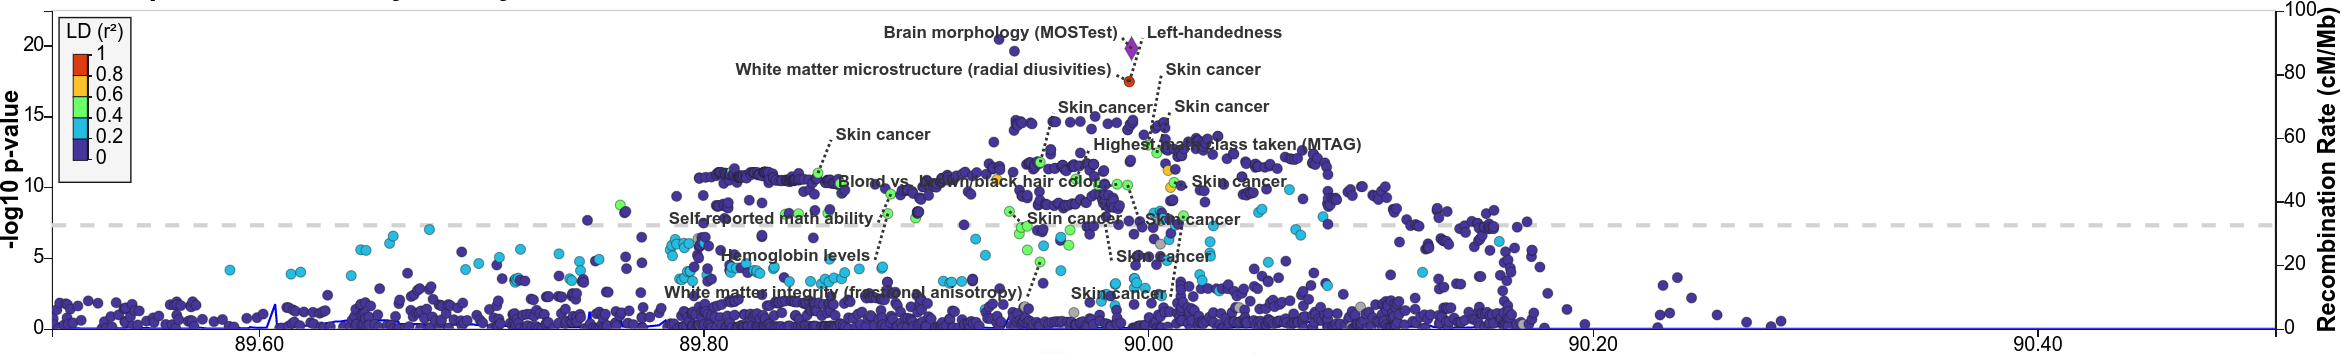
\includegraphics[width=\linewidth]{tubb3.png}
}
\par\medskip
\subfloat{
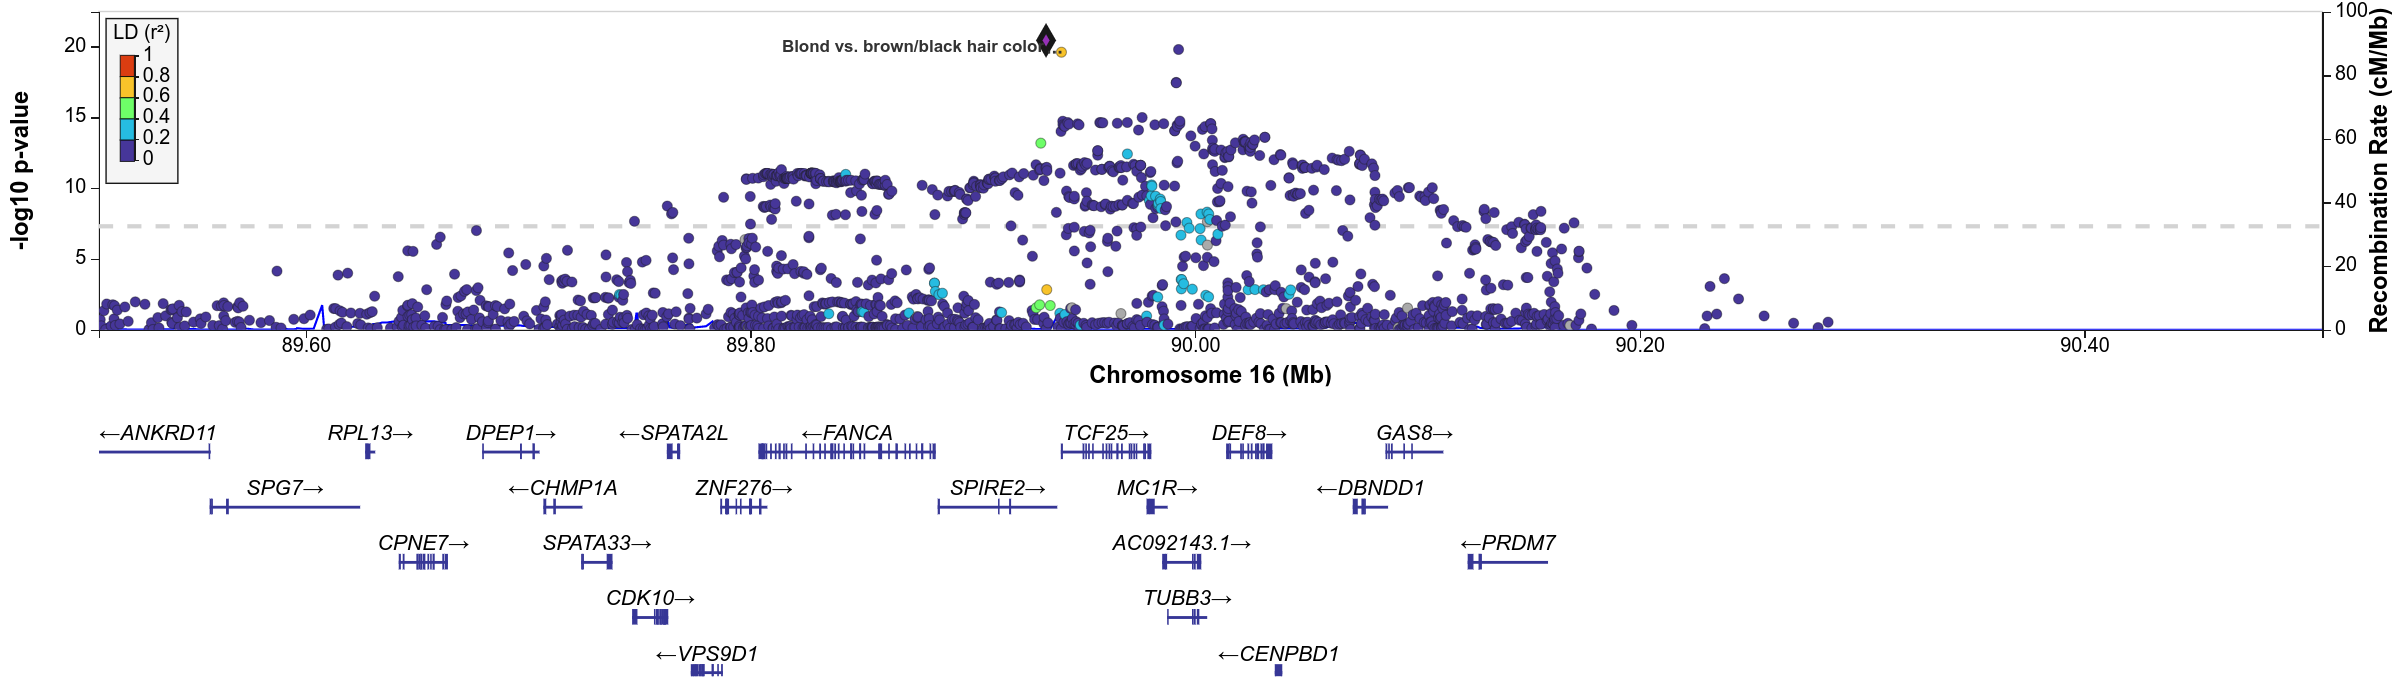
\includegraphics[width=\linewidth]{spire2.png}
}
\caption{Scores from the entire hemisphere \ac{gwas} for chromosome 16 TUBB3 and SPIRE2 lead \acp{snp} neighborhood. -log10P values, corresponding LD $r^2$ scores and cross-trait \acp{snp} annotations are shown, as retrieved by LocusZoom tool \cite{Boughton2021}. With a purple rhombus shape the point corresponding to the reference \ac{snp} for LD computation is displayed, rs111398992 (TUBB3) and rs72813426 (SPIRE2) on the top and middle graph respectively. At the bottom, a genes mapping, based on the GRCh37 build, is displayed for that region.}
\label{fig:chr16}
\end{adjustwidth}
\end{figure}


\section{Contributions}
In the current study, a detailed  data-driven multi-level analysis statistically elucidated the origins of cortical asymmetry, a complex multivariate phenotypic trait, on healthy individuals of European origin from the largest known \ac{mri} database to date, UK Biobank \cite{Littlejohns2020}. The degree to which plasticity effect is dispersed throughout the brain was statistically mapped using 2-way \ac{anova} and genetically quantified, through heritability studies. A coarse-to-fine data-driven segmentation identified homogeneously symmetric regions, without any prior anatomic knowledge.  Novel causal region-specific genetic variants were identified after \ac{mvgwas} on the derived partitions, complementing the existing literature \cite{Sha2021}. Different spatially-dependent genetic profiles were identified. Connections with biological pathways, concerning intra- and extra-cellular organization and the formation of symmetry axes, were made, by examining protein-protein interactions. The effect of a strong regulating, spatially dependent epigenetic effect on development was determined. Furthermore, gender-controlled epigenetic modifications appeared to affect cortical asymmetry. Gene- and \ac{snp}-level associative studies  with other genetically-driven traits led to the establishment of a tight genetic connection between  brain shape and asymmetry, while strong \ac{snp}-level genetic correlation was detected relatively to intellectual skills, handedness, \ac{ocd} and neuroticism. At the same time, computational acceleration was achieved, without observable loss in accuracy, through the application of simple operations, such as the average shape downsampling discussed in \autoref{sec:methods_on_pheno} that made the statistical analysis feasible, and the mean substitution of the \acp{snp}, that permitted a significant speed up of the \ac{cca} analysis.

\section{Limitations and possible extensions}
\subsection{Limitations}

\subsubsection{First stage}
Several limitations were detected during the conduction of this study, some of which could potentially be avoided by an extended future research. As far as the first stage of the analysis is concerned, lack of access to a test-retest dataset from UK Biobank and the disproportionate permutation spaces of 2-way \ac{anova} increased the error margin of the results, and the total variability of the data was not captured, because of the small sample size used, despite the three experimental iterations aggregation. In addition, covariates control prior to the statistical analysis could potentially provide a more consistent shape normalization and improve results quality. Furthermore, adaptive remeshing, by performing non-rigid group-wise registration, in place of the used naive method, would possibly have increased the results resolution, in exchange for greater computational demands.

\subsubsection{Second stage}
At the second stage, the absence of a signed statistic from \ac{mvgwas} did not allow to deduce whether identified \acp{snp}' presence contributes positively or negatively to cortical asymmetry, while also prohibiting the application of \ac{ldsc} during cross-trait analysis. Another step of multivariate regression, possibly in the form of \ac{cca}, using the lead \acp{snp} as covariates and the phenotype as predicted variable, could produce signed effects for each significant variant. 

Furthermore, 1000G project Phase 3 \ac{snp} filtering greatly reduced the amount of significant genes, with p-values lower than 5e-8, approximately by 82\% for the entire hemisphere \ac{gwas} (table \autoref{tab:1000g_entire_hemisphere} and \autoref{fig:1000g_entire_hemisphere}), while certain partitions lost all the \acp{snp} for at least one chromosome, whose p-value is lower than the Bonferroni threshold of 5e-8/31 (table \autoref{tab:1000g_lost_bonf_chr}). Although UK Biobank makes use of the 1000G Phase 3 project as the reference genome to perform phasing and imputation \cite{Bycroft2018}, in the current study, the high percentage of significant \ac{snp} pruning implies that non-significant \acp{snp} relationships are mostly driving the correlation studies and the LD score analysis.

It is also noteworthy to mention that the initial \ac{snp}-based filtering (cf. \autoref{sub:snpbased_filt}) has pruned away variants, which could potentially have a great impact on the studied phenotypic trait. However, studying the complementary case is difficult and highly error-prone, heavily relying on the sequencing technologies. Including rare variants and indels requires a denser genotyping, feasible through whole genome sequencing (WGS) \cite{Kierczak2022,Cirulli2020}, a technology to-be applied on UK Biobank anticipated dataset update \cite{Halldorsson2022}.


\subsection{Further extensions}
A possible extension would be to expand the gene-based meta-analysis on the entire set of identified partitions (i.e., not only on the second level ones), and develop a hierarchy-dependent \ac{gsea}, to promote cohesive results and remove false positives. Enriching the Spearman cross-trait correlation analyses with a larger amount and variety of traits' \ac{gwas} scores would, in addition, offer a better support of the identified correlations. Gender-based studies, that add gender as an additional covariate during  \ac{mvgwas}, could be used in a regression setting to derive the degree of variance explained by gender for each gene \cite{Rawlik2016}. Partitioned-based heritability analysis, centered at the regions of interest, could provide an answer to whether localized subpopulation structures exist. Lastly, modeling the cortical asymmetry heritability profile through epistasis analysis and even statistical shape modeling, extending existing ideas \cite{Filipe2019,Claes2014,White2020}, could make an approximate measurement of cortical plasticity in a spatially dependent manner possible, providing grounds for a personalized method of cortical structure anomaly detection and diagnosis of related diseases.


